%//==============================--@--==============================//%
\begin{theo}[\underline{Variável Aleatória (v.a.)}]{def:var-aleatoria}\label{def:var-aleatoria}
    Seja $(\Omega, \mathcal{A})$ um espaço mensurável. A função real $X$ diz-se uma variável aleatória (v.a.) se transformar o espaço de resultados $\Omega$ em $\mathbb{R}$ e a imagem inversa de qualquer conjunto de Borel de $\mathbb{R}$ for um evento $\sigma$-álgebra $\mathcal{A}$ definida sobre $\Omega$, i.e., $X: \Omega \mapsto \mathbb{R}$

    $$
        X^{-1} = \{\omega \in \Omega: X(\omega) \in B\} \in \mathcal{A},\, \forall B \in \mathcal{B}(\mathbb{R}) 
    $$
\end{theo}

\noindent\textbf{Tipo 1:} v.a. discreta --- tomam valores em conjuntos numeráveis de $\mathbb{R}$

\begin{mdframed}
$X$ diz se uma v.a. discreta caso exista um conjunto finito ou infinito numerável $D\, (D \subseteq \mathbb{R})$ tal que:
$$
    P(X \in D) = 1
$$
\end{mdframed}


\noindent\textbf{Tipo 2:} v.a. contínua --- tomam valores em intervalos de $\mathbb{R}$

\begin{mdframed}
   Sejam $X$ uma v.a. e $F_X = P(X \leq x),\, x \in \mathbb{R}$ a sua função de distribuição. $X$ diz-se uma v.a. contínua, caso:

   \begin{itemize}
       \item $F_X(x)$ seja uma função contínua
   \end{itemize}

   \noindent e exista uma função real de variável real $f_X(x)$ (função densidade probabilidade) que verifique:

   \begin{itemize}
       \item $f_X(x),\, \ge 0 \forall x \in \mathbb{R}$
       \item $F_X(x) = P(X \leq x) = \int_{-\infty}^x f_X(t)dt,\, \forall x \in \mathbb{R}$
   \end{itemize}

\noindent\textbf{Nota:} As últimas duas condições garantem a existência de uma função absolutamente contínua.
\end{mdframed}

%//==============================--@--==============================//%
\subsection[2.1 Função de (densidade) probabilidade]{\hspace*{0.075 em}\raisebox{0.2 em}{$\pmb{\drsh}$} Função de (densidade) probabilidade}

\noindent\textbf{Tipo 1:} A v.a. discreta $X$ com contradomínio $\mathbb{R}_X$ toma valores $x_i$ com probabilidades muito bem definidas. A sua caracterização somente se torna relevante se a par da indentificação do seu contradomínio adiantarmos os valores de $p_i$ para qualquer $x_i \in \mathbb{R}_X$:

\begin{theo}[\underline{Função de probabilidade }]{def:f.p.}\label{def:f.p.}
    A coleção de números $\{p_i\}$, que satisfazem

    \begin{itemize}
        \item $p_i = P(X = x_i) \ge 0$
        \item $\sum_i p_i = 1$
    \end{itemize}
    
    \noindent é designade de \textbf{função de probabilidade} da v.a. discreta $X$. Representaremos a f.p. de $X$ por:

    $$ 
    P(X = x_i)= \left\{
        \begin{array}{ll}
              p_i, & \text{se}\; x = x_i \in \mathbb{R}_X\\
               0, & \text{outros valores de }x\\
        \end{array} 
    \right. 
    $$
    
\end{theo}

\newpage
\noindent\textbf{Tipo 2:} para além das propriedades já anteriormente mencionados, a \textbf{função de densidade probabilidade} satisfaz:
{
\mdfsetup{linewidth=2pt}

\begin{mdframed}
$$
    \int_{-\infty}^{+\infty}f_X(x)dx = 1\qquad
    \int_{b}^{a}f_X(x)dx = P(a \leq x \leq b)
$$

\noindent Por sua vez, seja $X$ uma v.a. contínua, então:

\begin{itemize}
    \item $P(X = x) = 0,\, \forall x \in \mathbb{R}$, já que o evento ${X = x}$ é quase impossível.
    \item $P(a \leq x \leq b) = P(a < x \leq b) = P(a \leq x < b) = P(a < x < b)$
\end{itemize}

\noindent\textbf{Nota:} ao contrário da f.p. de uma v.a. discreta, a f.p. de uma v.a. contínua não é necessariamente limitada superiormente por 1.
\end{mdframed}
}
%//==============================--@--==============================//%
\subsection[2.1 Função de distribuição]{\hspace*{0.075 em}\raisebox{0.2 em}{$\pmb{\drsh}$} Função  de distribuição}

A função de distribuição representa a probailidade de uma dada v.a. $X$ tomar valores não superiores a um número real arbitrário $x$:

\begin{theo}[\underline{Função de distribuição }]{def:f.d.}\label{def:f.d.}
    A função de distribuição de uma v.a. $X$ é dada por
    $$ 
    F_X(x) = P(X \leq x) = P\left(x \in ]-\infty, x]\right),\, x \in \mathbb{R}
    $$  
\end{theo}

\noindent\textbf{Tipo 1:} A f.d. da v.a. discreta $X$ escreve-se "à custa" da f.p. de $X$:

\begin{align*}
    F_X(x) &= P(X \leq x)\\
           &= \sum_{\{x_i \in \mathbb{R}_X: x_i \leq x\}} P(X = x_i)\\
           &= \sum_{\{x_i \leq x\}} P(X = x_i),\, x_i \in \mathbb{R}_X
\end{align*}

\begin{theo}[\underline{Propriedades da função de distribuição uma v.a. discreta}]{def:prop-f.d.}\label{def:prop-f.d.}
Seja $X$ uma v.a. discreta com contradomínio $\mathbb{R}_X$. Então $F_X(x)$ é uma função:

\vspace{-0.5em}
\begin{itemize}
    \item em escada, com número de pontos de descontinuidade iguais aos valores  de $\mathbb{R}_X$.
    \item contínua à direita.
    \item monótona não decrescente de $x$.
    \item $0 \leq F_X(x) \leq 1$
    \item $F_X(-\infty) \to 0$ e $F_X(+\infty) \to 1$
    \item $P(X < x) = F_X(x^{-1}) = \lim_{h \to 0} F_X(x - h),\, h > 0$
    \item $P(a < X \leq b) = F_X(b) - F_X(a)$ e $P(a \leq X < b) = F_X(b^-) - F_X(a^-)$
    \item $P(a \leq X \leq b) = F_X(b) - F_X(a^-)$ e $P(a < X < b) = F_X(b^-) - F_X(a)$
    \item $P(X = x) = F_X(x) - F_X(x^-)$
\end{itemize}
\end{theo}

\newpage
\noindent\textbf{Tipo 2:} Tal como no caso discreto, a f.d. da v.a. contínua $X$ é dependente da função de probabilidade de $X$:

\begin{mdframed}
Seja $X$ uma v.a. contínua. Então, a sua f.d é dada por

$$
    F_X(x) = P(X \leq x) = \int_{-\infty}^x f_X(t)dt,\, x \in \mathbb{R}
$$
\end{mdframed}

\noindent\textbf{Nota:} Caso $F_X$ seja uma função absolutamente contínua e $f_X$ uma função contínua no ponto $x$ é possível obter a f.d.p derivando a f.d.:

$$
    f_X(x) = \dfrac{d F_X(x)}{dx}
$$

\begin{theo}[\underline{Propriedades da função de distribuição uma v.a. contínua}]{def:prop-f.d.-cont}\label{def:prop-f.d.-cont}
\noindent Seja $F_X(x)$ a f.d. da v.a. contínua $X$. Então $F_X(x)$ é uma função:


\begin{itemize} 
    \item contínua, à direira e à esquerda $F_X(x^+) = F_X(x^-),\, \forall x \in\mathbb{R}_X$.
    \item monótona não decrescente de $x$.
    \item $0 \leq F_X(x) \leq 1$
    \item $F_X(-\infty) \to 0$ e $F_X(+\infty) \to 1$
    \item $P(X \leq x) = P(X < x) = F_X(x)$
    \item $P(X > x) = 1 - F_X(x)$
\end{itemize}
\noindent Para $a$ e $b$:
\begin{align*}
    P(a \leq x \leq b) &= P(a < x \leq b) = P(a \leq x < b) = P(a < x < b)\\
    &= \int_a^b f_X(x)dx\\
    &= F_X(b) - F_X(a)
\end{align*}
\end{theo}

%//==============================--@--==============================//%
\subsection[2.2 Valor esperado, variância, moda e quantis]{\hspace*{0.075 em}\raisebox{0.2 em}{$\pmb{\drsh}$} Valor esperado, variância, moda e quantis}

A descrição completa do comportamento probabilístico está dependente de um conjunto de \textbf{parâmetros (indicador ou medida sumária)}:

\begin{itemize}
    \item \textbf{Localização central} --- valor esperado, moda, mediana.
    \item \textbf{Ordem} --- quantil de probabilidade
    \item \textbf{Dispersão} --- variância, desvio padrão e coeficiente de variação
\end{itemize}

\subsubsection[2.2.1 Valor esperado]{$\pmb{\rightarrow}$ Valor esperado}

\noindent \textbf{Tipo 1}: Se $E[X] = \sum_{|x| \in \mathbb{R}_X} x \cdot P(X = x) < +\infty$ (se a série for absolutamente convergente) o valor esperado de uma variável aleatória discreta $X$ com contradomínio $\mathbb{R}_X$ existe e é dada por:
$$
    \boxed{E[X] = \sum_{x \in \mathbb{R}_X} x \cdot P(X = x)}
$$

\noindent\textbf{Nota:} O valor esperado de uma v.a. discreta $X$ não pertence necessariamente ao conjunto de valores possíveis de $X$. Desta forma, é comum verificar $E(X) \notin \mathbb{R}_X$.

\vspace{1 em}
\noindent \textbf{Tipo 2}: A definição do valor esperado no caso contínuo é análogo ao discreto. Onde tínhamos $\sum$ e $P(X = x)$ passamos a ter $\int$ e $f_X(X)$. O valor esperado da v.a. contínua é igual a:
$$
    E[X] = \int_{-\infty}^{+\infty} x \cdot f_X(x) dx
$$
\noindent Desde que o integral seja absolutamente convergente ($\int_{-\infty}^{+\infty} |x| \cdot f_X(x) dx < -\infty$).

\begin{theo}[\underline{Propriedades do valore esperado}]{def:prop-v.e.}\label{def:prop-v.e.}
\noindent O valore esperado satisfaz as seguintes propriedades:

\begin{enumerate} 
    \item $E[b] = b,\, b\in \mathbb{R}$.
    \item $E[aX + b] = aE[X] + b,\, b,a\in \mathbb{R}$.
    \item Seja $Y = \Omega(X)$ uma v.a., função da v.a. discreta $X$. Então, caso $E(Y)$ exista:
    $$
        E(Y) = E(\Omega(X)) = \sum_x \Omega(X) \cdot P(X = x)
    $$

    De forma análoga, se considerarmos o caso contínuo:
    $$
        E(Y) = E(\Omega(X)) = \int_{-\infty}^{+\infty} \Omega(X) \cdot P(X = x)
    $$

    De um modo geral, $E(\Omega(X)) \ne \Omega(E[X])$
\end{enumerate}
\end{theo}

\subsubsection[2.2.2 Moda]{$\pmb{\rightarrow}$ Moda}
\noindent A moda corresponde ao ponto máximo da função de probabilidade (no caso discreto) ou função de densidade probabilidade (no caso contínuo):

\begin{align*}
    &\textbf{tipo 1:}\; mo: P(mo) = \underset{x}{max} f_X(x)\\
    &\textbf{tipo 2:}\; mo: P(X = mo) = \underset{x}{max} P(X = x)\\
\end{align*}

\subsubsection[2.2.2 Mediana]{$\pmb{\rightarrow}$ Mediana}

{
\mdfsetup{linewidth=2pt}

\begin{mdframed}
    \noindent A mediana de uma v.a. $X$ é todo e qualquer ponto:
    $$
    me: me(X): \dfrac{1}{2} \leq F_X(me) \leq \dfrac{1}{2} + P(X = me)
    $$
    
    \noindent Como no caso contínuo $P(X = me) = 0$ a fórmula reduz-se a:
    $$
        me: me(X): \leq F_X(me) = \dfrac{1}{2}
    $$
\end{mdframed}
}

\subsubsection[2.2.2 Quantil de probabilidade]{$\pmb{\rightarrow}$ Quantil de probabilidade}
\begin{theo}[\underline{Quantil de probabilidade de $p$ de v.a. discreta}]{def:quantil}\label{def:quantil}
    O quantil de probabilidade $p$ ($0 < p < 1$) da v.a. X é representado por $\mathcal{X}_p$ e satisfaz

    $$
        \mathcal{X}_p: p \leq F(\mathcal{X}_p) \leq p + P(X = \mathcal{X}_p)
    $$

    No caso contínuo:

    $$
        \mathcal{X}_p: F(\mathcal{X}_p) = p 
    $$  
\end{theo}

\subsubsection[2.2.3 Variância]{$\pmb{\rightarrow}$ Variância}

\noindent A variância define o grau de dispersão dos valores de uma dada v.a. em torno do seu centro da gravidade:

\begin{theo}[\underline{Variância}]{def:var}\label{def:var}
\noindent A variância é dada por:
    \begin{align*}
        V(X) = E\{[X - E(X)]^2\} &= E\{[X^2 - 2X^2E(X) + E(X)^2]\}\\
        &= E(X)^2 + E(X^2) + E[-2XE(X)]\\
        &= E(X)^2 + E(X^2) + -2E(X)E(X)\\
        &= E(X^2) - E(X)^2 
    \end{align*}

\noindent e satisfaz as seguintes propriedades:

\begin{enumerate} 
    \item $E(b) = 0,\, b\in \mathbb{R}$.
    \item $E(aX + b) = a^2V(X),\, b,a\in \mathbb{R}$.
    \item $V(X) \ge 0$, qualquer que seja a v.a. $X$
\end{enumerate}
\end{theo}

\subsubsection[2.2.4 Desvio Padrão]{$\pmb{\rightarrow}$ Desvio Padrão}

\noindent É costume recorrer a outra medida de dispersão absoluta, já que a variância não é expressa nas mesmas unidades que a variável aleatória. O \textbf{desvio padrão} trata-se da raiz quadrada positiva da variância de $X$:

$$
    \boxed{DP(X) = + \sqrt{V(X)}}
$$

\noindent Independente de $X$ ser discreta ou contínua.

\subsubsection[2.2.5 Coeficiente de variação]{$\pmb{\rightarrow}$ Coeficiente de variação}

\noindent \textbf{O coeficiente de variação} é uma medida de dispersão relativa, adimensional, que permite comparar a dispersão das distribuições com localizações (ou ordens de grandeza) distintas. É dada por:

$$
    \boxed{CV(X) = \dfrac{DP(X)}{E(X)}}
$$
\noindent Independente de $X$ ser discreta ou contínua e desde que $E[X] \ne 0$. 

%//==============================--@--==============================//%
\subsection[2.1 Distribuições discretas conhecidas]{\hspace*{0.075 em}\raisebox{0.2 em}{$\pmb{\drsh}$} Distribuições discretas conhecidas}

\subsubsection[2.2.3 Distribuições discretas]{$\pmb{\rightarrow}$ Distribuições discretas}

\noindent \textbf{Distribuição uniforme discreta} --- Esta distribuição é razoável quando a v.a. discreta toma $n$ valores distintos, todos com a mesma probabilidade. Sem perda de generalidade, considera-se que esta v.a. toma $n$ valores distintos, $x_1,x_2,\dots,x_n$ em que $x_1 < x_2 < \dots < x_n$.

\begin{theo}[\underline{Distribuição Uniforme Discreta}]{def:unif}\label{def:unif-disc}
\noindent A v.a. discreta $X$ diz-se ter distribuição uniforme discreta no conjunto $\{x_1,x_2, \dots, x_n\}$, se a sua f.p. coincidir com a que conta na tabela abaixo:

\vspace{1 em}
\begin{center}
\begin{tabular}{p{4cm}p{8cm}}
\toprule
\textbf{Notação} & $X \sim \text{uniforme discreta}(\{x_1,x_2, \dots, x_n\})$\\
\addlinespace
\textbf{Parâmetro} & $\{x_1,x_2, \dots, x_n\}$ $(x_i \in \mathbb{R}, i = 1, \dots, n)$\\
\addlinespace
\textbf{Contradomínio} & $\{x_1,x_2, \dots, x_n\}$\\
\addlinespace
\textbf{F.p} & $P(X = x)= \left\{
                                \begin{array}{ll}
                                      \frac{1}{n}, & x = x_i \in \mathbb{R}_X\\
                                       0, & \text{c.c.}\\
                                \end{array} 
                          \right.$\\
\addlinespace
\textbf{Valor Esperado} & $E(X) = \frac{1}{n}\sum_{i = 1}^{n} x_i$\\
\addlinespace
\textbf{Variância} & $V(X) = \frac{1}{n}\sum_{i = 1}^{n} x_i^2 - (\frac{1}{n}\sum_{i = 1}^{n} x_i)^2$\\
\bottomrule
\end{tabular}
\end{center}

\vspace{0.5 em}
\end{theo}

\noindent As duas subsequentes distribuições estão dependentes da definição de \textbf{prova de Bernoulli} --- Uma experiência aleatória diz-se uma prova de Bernoulli se possuir apenas dois resultados possíveis:
\begin{itemize}
    \item Um sucesso, que ocorre com probabilidade $p$ $(0 \leq p \leq 1)$
    \item Um insucesso, que ocorre com probabilidade $(1 - p)$
\end{itemize}

\vspace{-0.85em}
\begin{theo}[\underline{Distribuição de Bernoulli}]{def:bernoulli-dist}\label{def:bernoulli-dist}
    \noindent Porventura, a v.a. discreta
    \begin{itemize}
        \item $X =$ número de sucessos numa prova de Bernoulli
    \end{itemize}
    
    \noindent diz-se com \textbf{Distribuição de Bernoulli} com parâmetro $p$ e possui a f.p. na seguinte tabela:
    
    \begin{center}
    \begin{tabular}{p{4cm}p{8cm}}
    \toprule
    \textbf{Notação} & $X \sim \text{Bernoulli}(p)$\\
    \addlinespace
    \textbf{Parâmetro} & $p = P(\text{sucesso})$ $(p \in [0,1])$\\
    \addlinespace
    \textbf{Contradomínio} & $\{0,1\}$\\
    \addlinespace
    \textbf{F.p} & $P(X = x)= \left\{
                                    \begin{array}{ll}
                                          p^x(1 - p)^{1-x}, & x = 0,1\\
                                           0, & \text{c.c.}\\
                                    \end{array} 
                              \right.$\\
    \addlinespace
    \textbf{Valor Esperado} & $E(X) = p$\\
    \addlinespace
    \textbf{Variância} & $V(X) = p(1-p)$\\
    \bottomrule
    \end{tabular}
    \end{center}

    \vspace{0.35em}
\end{theo}

\newpage
\noindent \textbf{Distribuição Binomial} --- É pertinente saber qual a distribuição do número de sucessos num número fixo $n$ de provas de Bernoulli realizadas de forma independente e com probabilidade de sucesso comum $p$.

\begin{theo}[\underline{Distribuição binomial}]{def:bin}\label{def:bin}
\noindent A v.a. discreta

\begin{itemize}
    \item $X =$ número de sucessos num conjunto de $n$ provas de Bernoulli independentes com probabilidade de sucesso comum e igual a $p$
\end{itemize}

\noindent diz-se com distribuição binomial de parâmetros $(n,p)$ e possui a f.p. que consta na seguinte tabela:

\vspace{1 em}
\begin{center}
\begin{tabular}{p{4cm}p{8cm}}
\toprule
\textbf{Notação} & $X \sim \text{binomial}(n,p)$\\
\addlinespace
\textbf{Parâmetro} & $\begin{aligned}
                            &n = \text{número de provas de Bernoulli}\; (n \in \mathbb{N}_0)\\
                            &p = P(\text{sucesso})\; (p \in [0,1])
                     \end{aligned}$\\
\addlinespace
\textbf{Contradomínio} & $\{0,1, \dots, n\}$\\
\addlinespace
\textbf{F.p} & $P(X = x)= \left\{
                                \begin{array}{ll}
                                      \binom{n}{x}p^x(1 - p)^{n-x}, & x = 0,1\\
                                       0, & \text{c.c.}\\
                                \end{array} 
                          \right.$\\
\addlinespace
\textbf{Valor Esperado} & $E(X) = np$\\
\addlinespace
\textbf{Variância} & $V(X) = np(1 - p)$\\
\bottomrule
\end{tabular}
\end{center}

\vspace{1 em}
\noindent \textbf{Propriedade} --- Seja $Y$ o número de insucessos em $n$ provas de Bernoulli ($Y = n - X$)

\vspace{-1 em}
\begin{align*}
    Y &= n - X \sim binomial(n, 1 - p)\\[4pt]
    F_Y(y) &= P(n - X \leq y)\\
    &= P(X \ge n - y)\\
    &= 1 - P(X < n - y)\\
    &= 1 - P(X \leq n - y - 1)\\
    &= 1 - F_X(n - y - 1)
\end{align*}
\vspace{0.5 em}
\end{theo}

\newpage
\noindent \textbf{Distribuição geométrica} --- Caso estejamos interessados em contabilizar o número total de provas de Bernoulli realizadas até ao registo do primeiro sucesso, passamos a lidar com uma v.a. com distribuição geométrica.

\begin{theo}[\underline{Distribuição geométrica}]{def:geom}\label{def:geom}
\noindent A v.a. discreta

\begin{itemize}
    \item $X =$ número de provas de Bernoulli (independentes com probabilidade de sucesso comum e igual a $p$) até à ocorrência do primeiro sucesso.
\end{itemize}

\noindent diz-se com distribuição geométrica de parâmetro $p$ e possui a f.p. que consta na seguinte tabela:

\vspace{1 em}
\begin{center}
\begin{tabular}{p{4cm}p{8cm}}
\toprule
\textbf{Notação} & $X \sim \text{geométrica}(p)$\\
\addlinespace
\textbf{Parâmetro} & $p = P(\text{sucesso})$ $(p \in [0,1])$\\
\addlinespace
\textbf{Contradomínio} & $\{1,2, \dots, n\}$\\
\addlinespace
\textbf{F.p} & $P(X = x)= \left\{
                                \begin{array}{ll}
                                       p(1 - p)^{x-1}, & x = 0,1\\
                                       0, & \text{c.c.}\\
                                \end{array} 
                          \right.$\\
\addlinespace
\textbf{Valor Esperado} & $E(X) = \frac{1}{p}$\\
\addlinespace
\textbf{Variância} & $V(X) = \frac{1 - p}{p^2}$\\
\bottomrule
\end{tabular}
\end{center}

\noindent \textbf{Falta de memória da distribuição geométrica} --- Seja $X \sim \text{geométrica}(p)$. Então,

$$
    \boxed{P(X > k + x | X > k) = P(X > x),\, \forall k,x \in \mathbb{N}}
$$

\noindent De modo equivalente, a v.a. $(X - k | X > k)$ que representa o número de provas adicionais, sabendo que não se registou qualquer sucesso nas primeiras k provas, também possui distribuição geométrica com parâmetro $p$:

$$
\boxed{(X - k | X > k) \sim \text{geométrica}(p),\, k \in \mathbb{N}}
$$

\noindent Esta propriedade traduz um \textbf{recomeço probabilístico}. A informação acerca da não ocorrência de sucessos nas primeira $k$ provas de Bernoulli não é relevante para os cálculos subsequentes.

\vspace{0.5 em}
\end{theo}

\newpage
\noindent\textbf{Distribuição Poisson} --- Frequentemente usada na contagem de ocorrências de certo tipo de eventos em periodos fixos de tempo, áreas, volumes ... Eventos tais como chegadas, acidentes, falhas de equipamento, testemunhos verdadeiros em tribunal, etc.

\begin{theo}[\underline{Distribuição poisson}]{def:poisson}\label{def:poisson}
\noindent A v.a. $X$ diz-se com distribuição de Poisson e parâmetro $\lambda$ caso possua f.p. na tabela seguinte:

\vspace{1 em}
\begin{center}
\begin{tabular}{p{4cm}p{8cm}}
\toprule
\textbf{Notação} & $X \sim \text{Poisson}(\lambda)$\\
\addlinespace
\textbf{Parâmetro} & $\lambda$ $(\lambda \in \mathbb{R}^+)$\\
\addlinespace
\textbf{Contradomínio} & $\mathbb{N}_0$\\
\addlinespace
\textbf{F.p} & $P(X = x)= \left\{
                                \begin{array}{ll}
                                       e^{-\lambda}\frac{\lambda^x}{x!}, & x = 0,1,2 \dots\\
                                       0, & \text{c.c.}\\
                                \end{array} 
                          \right.$\\
\addlinespace
\textbf{Valor Esperado} & $E(X) = \lambda$\\
\addlinespace
\textbf{Variância} & $V(X) = \lambda$\\
\bottomrule
\end{tabular}
\end{center}

\noindent\textbf{Nota:} Se porventura procurarmos a distribuição da expansão ou contração da unidade para a qual é realizada a contagem de ocorrências, basta multiplicar o parâmetro $\lambda$ pelo coeficiente da transformação em causa.
\end{theo}

\noindent\textbf{A aproximação de Poisson da distribuição binomial} --- A pertinência desta aproximação prende-se com o facto de nem sempre ser possível calcular a probabilidade de certos eventos recorrendo às tabelas disponíveis:

\vspace{1 em}
\noindent A f.p. da v.a. $X \sim$binomial($np$) pode ser aproximada satisfatoriamente pela f.p./f.d. da v.a. aproximativa

$$
    \Tilde{X} \sim \text{Poisson}(np),\qquad \text{quando } n > 20 \text{ e } p < 0.1
$$

\noindent já que

$$
    \underset{np = \lambda \text{ fixo}}{\underset{p \to 0}{\underset{n \to +\infty}{\lim}}} \binom{n}{x}p^x(1 - p)^{n-x} = e^{-\lambda}\frac{\lambda^x}{x!}
$$

\noindent Adianta-se também que:

$$
    \sum_{x = 0}^{+\infty} \left|\binom{n}{x}p^x(1 - p)^{n-x} - e^{-\lambda}\frac{\lambda^x}{x!}\right| \leq 2p,\;\: \text{para $0 \leq p \leq 1$}
$$


%//==============================--@--==============================//%
\newpage
\subsubsection[2.2.3 Distribuições contínuas]{$\pmb{\rightarrow}$ Distribuições contínuas}

\noindent \textbf{Distribuição uniforme contínua} --- Esta distribuição é o análogo da distribuição uniforme discreta. Não surpreende que se trate de uma distribuição adequada a descrever o comportamento probabilístico de uma v.a. cujos valores possíveis se crê terem todos o mesmo peso.

\begin{theo}[\underline{Distribuição Uniforme Contínua}]{def:unif-cont}\label{def:unif-cont}
\noindent A v.a. contínua $X$ diz-se ter distribuição uniforme contínua no intervalo $[a,b]$, se a sua f.p. coincidir com a que conta na tabela abaixo:

\vspace{1 em}
\begin{center}
\begin{tabular}{p{4cm}p{8cm}}
\toprule
\textbf{Notação} & $X \sim \text{uniforme}(a,b)$\\
\addlinespace
\textbf{Parâmetro} & $\begin{aligned}
                        &a\, \text{extremo inferior do intervalo; }a \in \mathbb{R}\\
                        &b\, \text{extremo superior do intervalo; }b \in \mathbb{R}
                     \end{aligned}$\\
\addlinespace
\textbf{Contradomínio} & $[a,b]$\\
\addlinespace
\textbf{F.d.p} & $f_X(x) = \left\{
                                \begin{array}{ll}
                                      \frac{1}{b - a}, & xa \leq x \leq b\\
                                       0, & \text{c.c.}\\
                                \end{array} 
                          \right.$\\
\addlinespace
\textbf{Valor Esperado} & $E(X) = \frac{a + b}{2}$\\
\addlinespace
\textbf{variância} & $V(X) = \frac{(a + b)^2}{12}$\\
\bottomrule
\end{tabular}
\end{center}

\noindent\textbf{Propriedade} --- Considere-se que $X \sim \text{uniforme}(a,b)$. Então , os intervalos --- com a mesma amplitude e contidos em $[a,b]$ --- são equiprováveis.
\vspace{0.5 em}
\end{theo}


\noindent \textbf{Distribuição Normal} --- Esta distribuição surge associada à modelação de observações relativas a medições de temperaturas, velocidades, erros, volumes de ruído, etc. Surge também como distribuição aproximada, nomeadamente de algumas distribuições discretas, ou ainda, de médias aritméticas ou somas de v.a.

\begin{theo}[\underline{Distribuição Normal}]{def:norm}\label{def:norm}
\noindent A v.a. contínua $X$ diz-se ter distribuição normal de parâmetros $\mu$ e $\sigma^2$ caso possua a seguinte f.d.p:

\vspace{1 em}
\begin{center}
\begin{tabular}{p{4cm}p{8cm}}
\toprule
\textbf{Notação} & $X \sim \text{normal}(\mu,\sigma^2)$\\
\addlinespace
\textbf{Parâmetro} & $\begin{aligned}
                        &\mu\, (\mu \in \mathbb{R})\\
                        &\sigma^2\, (\sigma^2 \in \mathbb{R}^+)
                     \end{aligned}$\\
\addlinespace
\textbf{Contradomínio} & $\mathbb{R}$\\
\addlinespace
\textbf{F.d.p} & $f_X(x)= \frac{1}{\sqrt{2 \pi} \sigma}e^{-\frac{(x - \mu)^2}{2\sigma^2}},\,\; -\infty < x < +\infty$\\
\addlinespace
\textbf{Valor Esperado} & $E(X) = \mu$\\
\addlinespace
\textbf{Variância} & $V(X) = \sigma^2$\\
\bottomrule
\end{tabular}
\end{center}

\vspace{0.5 em}
\end{theo}

\noindent \textbf{F.d.p da v.a. normal} --- A f.d.p da v.a. normal é simétrica em torno de $\mu$ e tem forma de sino. É devido a estes dois factos que a mediana é igual à moda e ao valore esperado:
$$
    \boxed{me(X) = mo(X) = E(X) = \mu}
$$
\noindent O valor de $\sigma^2$, como seria de esperar, determina o achatamento da f.d.p. desta v.a.:
\begin{itemize}
    \item $\sigma^2$ pequeno, f.d.p muito alongada
    \item $\sigma^2$ grande, f.d.p muito achatada
\end{itemize}

\noindent \textbf{F.d. da v.a. normal} --- A f.d. da v.a. normal é dada por:

$$
    \int_{-\infty}^x \dfrac{1}{\sqrt{2 \pi} \sigma}e^{-\dfrac{(x - \mu)^2}{2\sigma^2}}dt,\,\; -\infty < x < +\infty
$$

\noindent Não possui expressão fechada, pelo que só pode ser obtida numericamente.

{
\mdfsetup{linewidth=2pt}

\begin{mdframed}
    \noindent \textbf{Distribuição Normal Padrão} --- Seja $X \sim \text{normal}(\mu,\sigma^2)$. Então, recorrendo ao processo de estandarização:
    
    \vspace{-0.5em}
    \begin{align*}
        Z &= \dfrac{X - E(X)}{\sqrt{V(X)}} = \dfrac{X - \mu}{\sigma} \sim \text{normal}(0,1)\\
        F_Z(z) &= P(Z \leq z) = \int_{-\infty}^x \frac{1}{\sqrt{2 \pi}}e^{-\frac{y^2}{2}}dy = \Phi(z)
    \end{align*}
    
    \noindent $Z$ possui \textbf{distribuição normal padrão}. É à custa de $Z$ que se obtém a f.d. da v.a. $X \sim \text{normal}(\mu,\sigma^2)$, para quaisquer valores admissíveis de $\mu$ e $\sigma^2$

    $$
        F_X(x) = P(X \leq x) = P\left(Z = \dfrac{X - \mu}{\sigma} \leq \dfrac{x - \mu}{\sigma}\right) = \Phi\left(\dfrac{x - \mu}{\sigma}\right)
    $$

    \noindent\textbf{Nota:} Graças à simetria da f.p.d. da normal padrão em torno da origem, podemos concluir que
    $$
        \Phi(-z) = 1 - \Phi(z),\, -\infty < x < +\infty
    $$
\end{mdframed}
}

\vspace{1.5em}
\begin{figure}[H]
    \centering
    \resizebox{0.875\textwidth}{!}{%
        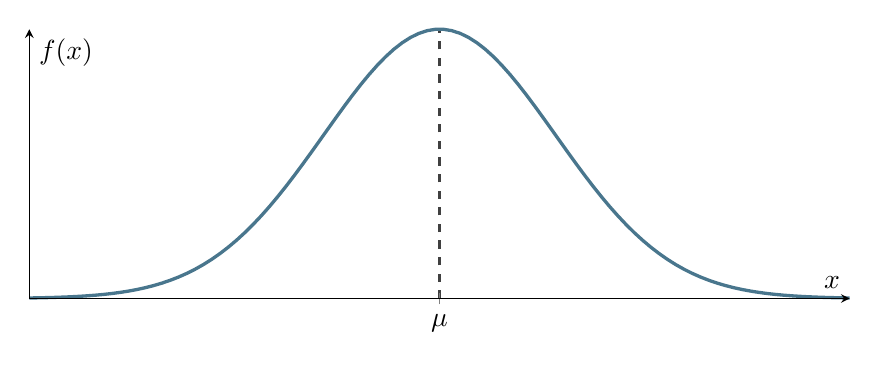
\begin{tikzpicture}
            \begin{axis}[
                no markers, 
                domain=0:10, 
                samples=100,
                ymin=0,
                axis lines*=left, 
                xlabel=$x$,
                ylabel=$f(x)$,
                height=5cm, 
                width=12cm,
                xtick={5}, 
                xticklabels={$\mu$},
                ytick=\empty,
                enlargelimits=false, 
                clip=false, 
                axis on top,
                axis lines = middle
            ]
            
            \addplot [very thick,cyan!50!black] {1/(2*sqrt(pi))*exp(-((x - 5)^2)/4)};
    
            \addplot +[mark=none,thick,color=darkgray,dashed] coordinates {(5, 0) (5, 0.28)};
            \end{axis}
        \end{tikzpicture}
    }
    \caption{Função Densidade de Probabilidade (f.d.p) da Distribuição Normal --- normal$(\mu,\sigma^2)$}
\end{figure}


%//==============================--@--==============================//%
\newpage
\noindent \textbf{Distribuição exponencial} --- É a distribuição mais utilizada na caracterização da duração de equipamento, naquilo que usualmente é designado por \textit{testes de vida}.

\begin{theo}[\underline{Distribuição exponencial}]{def:exp}\label{def:exp}
    \noindent A v.a. contínua $X$ diz-se ter distribuição exponencial de parâmetro $\mu$ caso possua a seguinte f.d.p:

    \vspace{0.5 em}
    \begin{center}
        \begin{tabular}{p{4cm}p{8cm}}
            \toprule
            \textbf{Notação} & $X \sim \text{exponencial}(\lambda)$\\
            \addlinespace
            \textbf{Parâmetro} & $\lambda\; (\lambda \in \mathbb{R}^+)$\\
            \addlinespace
            \textbf{Contradomínio} & $\mathbb{R}^+_0$\\
            \addlinespace
            \textbf{F.d.p} & $f_X(x)= \lambda e^{-\lambda x},\,\; x \ge 0$\\
            \addlinespace
            \textbf{Valor Esperado} & $E(X) = \frac{1}{\lambda}$\\
            \addlinespace
            \textbf{Variância} & $V(X) = \frac{1}{\lambda^2}$\\
            \bottomrule
        \end{tabular}
    \end{center}

    \noindent \textbf{Falta de memória da distribuição exponencial} --- Seja $X \sim \text{exponencial}(\lambda)$. Então,

    \vspace{-1 em}
    \begin{align*}
        P(X \leq t + x | X > t)\; &=\; P(X \leq x),\, \forall t,x \in \mathbb{R}^+_0\\
        P(X > t + x | X > t)\; &=\; P(X > x),\, \forall t,x \in \mathbb{R}^+_0\\
        (X - t | X > t)\; &\sim\; \text{exponencial}(\lambda),\, t \in \mathbb{R}^+_0
    \end{align*}

    \noindent Ao considerarmos que $X$ representa a vida de um item e que $X$ tem distribuição exponencial$(\lambda)$, a vida residual no instante $t$, $(X - t | X > t)$ possuirá a mesma distribuição e o mesmo parâmetro de $X$.
    
\vspace{0.5 em}
\end{theo}

\noindent\textbf{Relação entre as distribuições exponencial e de Poisson} --- Sejam:

\begin{itemize}
    \item $N_t$ o número de ocorrências de um evento no intervalo $]0,t],\, t > 0$
    \item $X_i$ o tempo entre ocorrências consecutivas $(i -1)$ e $i$ do evento
\end{itemize}

\noindent Caso a coleção de v.a. $\{N_t, t > 0\}$ seja um processo de Poisson de taxa $\lambda$, é sabido que $N_t \sim \text{Poisson}(\lambda t)$ e podemos concluir que

$$
    \boxed{X_i \overset{i.i.d}{\sim} \text{exponencial}(\lambda),\; i \in \mathbb{N}}
$$

\noindent O de $\overset{i.i.d}{\sim}$ lê-se \textit{independentes e identicamente distribuídos a}

\begin{figure}[H]
    \centering
    \begin{tikzpicture}
    \begin{axis}[
        no markers, 
        domain=0:5, 
        samples=100,
        ymin=0,
        ymax=2,
        axis lines*=left, 
        xlabel=$x$,
        ylabel=$f(x)$,
        ylabel style={at={(axis description cs:-0.1,.5)},anchor=south},
        height=6cm, 
        width=12cm,
        xtick=\empty, 
        ytick={1.5},
        yticklabels={$\lambda$},
        enlargelimits=false, 
        clip=false, 
        axis on top,
        axis lines = middle
    ]
    \addplot [very thick,cyan!50!black] {1.5*exp(-1.5*x)};
    \end{axis}
    \end{tikzpicture}
     \caption{Função Densidade de Probabilidade (f.d.p) da Distribuição Exponencial --- exponencial$(\lambda)$}
\end{figure}

%//==============================--@--==============================//%